\subsection{Wait, What Happened to My Rectangles?}

When most of us first learned integration, we were told a comforting story.

You have a function. You want to find the area under the curve. So you chop it into little rectangles, add them up, and as the rectangles get thinner, your approximation becomes exact. Voilà! Calculus.

This is Riemann integration. And it worked great—for a while.

But then math got ambitious. We started asking harder questions. What happens when your function isn’t continuous? What if it has too many jumps? What if your data isn’t spread along a line but scattered across weird, fragmented sets? What if your function is technically defined everywhere but behaves so badly that stacking rectangles becomes meaningless?

That’s when the rectangles stopped working.

Riemann’s beautiful method collapsed under the weight of pathological examples. Functions that were defined everywhere but continuous nowhere. Sets that were uncountably infinite but had zero length. Attempts to make sense of infinite sums that led to contradictions.

And that’s when Henri Lebesgue entered the scene.

He didn’t try to patch the rectangle-stacking method. He scrapped it entirely and started over—from the ground up.

Instead of slicing the \textit{domain} (the x-axis), Lebesgue sliced the \textit{range}. He grouped together all the parts of the domain where the function takes on a particular value, then measured the “size” of those parts. His idea wasn’t to build an area by stacking shapes—it was to \textbf{assign size to sets} in a consistent, flexible way, and then use that to integrate.

In doing so, Lebesgue didn’t just invent a new technique—he invented a new worldview. He introduced the concept of a \textit{measure}: a general way of quantifying how big, or small, or strange a set is. And suddenly, all those freakish, fragmented, nightmare-inducing functions could be handled in a calm, orderly framework.

Riemann had drawn with rulers. Lebesgue brought a flashlight and said: “Let’s measure wherever the light lands.”

This wasn’t a refinement. It was a full-blown revolution.

Thomas Kuhn, the philosopher of science, described these moments as \textbf{paradigm shifts}—when the old rules stop working and a new framework has to take over. Mathematics doesn’t evolve smoothly. It breaks. And then it rebuilds itself, stranger and stronger than before.

\begin{quote}
\textbf{Sometimes math doesn’t evolve. It shatters. And this was one of those moments.}
\end{quote}

And that brings us to this little conversation:

\begin{figure}[H]
\centering
\begin{tikzpicture}[every node/.style={font=\footnotesize}]

% Panel 1 — student struggling with abstraction
\comicpanel{0}{4}
  {Student}
  {Lebesgue}
  {I miss Riemann. He let me stack rectangles. You just give me this weird $\int f\, d\mu$ thing.}
  {(-0.6,-0.5)}

% Panel 2 — Lebesgue explains calmly
\comicpanel{6.5}{4}
  {Student}
  {Lebesgue}
  {That's because I’m measuring over messy sets instead of neat intervals. Welcome to the deep end.}
  {(.55,-0.5)}

% Panel 3 — student is clearly panicking
\comicpanel{0}{0}
  {Student}
  {Lebesgue}
  {Wait... some of these “sets” don’t even feel like numbers anymore. Am I still doing math?}
  {(-0.65,-0.6)}

% Panel 4 — Lebesgue smirks
\comicpanel{6.5}{0}
  {Student}
  {Lebesgue}
  {Notation didn’t get weird. Reality did.}
  {(0.75,-0.6)}

\end{tikzpicture}
\caption{Lebesgue integration: it’s not just a different notation; it’s a different universe.}
\end{figure}

And if you’ve ever stared at \( \int f \, d\mu \) in a machine learning paper and felt your stomach drop—you’re not alone. You’ve just stumbled into one of the most profound moments in mathematical history.



